% Created 2023-08-26 Sat 18:02
% Intended LaTeX compiler: pdflatex
\documentclass[11pt]{article}
\usepackage[utf8]{inputenc}
\usepackage[T1]{fontenc}
\usepackage{graphicx}
\usepackage{longtable}
\usepackage{wrapfig}
\usepackage{rotating}
\usepackage[normalem]{ulem}
\usepackage{amsmath}
\usepackage{amssymb}
\usepackage{capt-of}
\usepackage{hyperref}
\usepackage{tikz, array, pgfplots, xcolor}
\author{Hankertrix}
\date{\today}
\title{Math Module 1A Lecture Notes}
\hypersetup{
 pdfauthor={Hankertrix},
 pdftitle={Math Module 1A Lecture Notes},
 pdfkeywords={},
 pdfsubject={},
 pdfcreator={Emacs 29.1 (Org mode 9.6.6)}, 
 pdflang={English}}
\begin{document}

\maketitle
\setcounter{tocdepth}{2}
\tableofcontents

\newpage


\section{Sets}
\label{sec:org2925294}
A set is basically just a collection of objects, and the objects inside a set are called elements, or points. To say that \(x\) is an element of set \(A\) is represented by \(x \in A\) or \(A \ni x\). Similarly, to say that \(x\) is not an element of set \(A\) is represented by \(x \notin A\). A set is usually described using curly braces \(\{\}\).
\\[0pt]

Examples:

\[A = \{1,2,3\} \rightarrow 1 \in A, 2 \in A, 3 \in A, 4 \notin A, \pi \notin A\]
\[B = \{\text{Homer}, \text{Marge}, \text{Bart}, \text{Lisa}, \text{Maggie}\}\]
\[\text{Homer}\in B, 1 \notin B, \text{Ned Flanders} \notin B\]


\subsection{Describing sets}
\label{sec:orgcb4e38c}

Common ways to describe sets include:

\[A = \{x: \text{some condition}\}\]
\[\text{A is the set of objects x for which the condition is true.}\]
\[B = \{x \notin B: \text{some condition}\}\]
\[\text{B is the set of objects x in Set B for which the condition is true}\]
\\[0pt]
Examples:

\[\mathbb{Z} = \{x: \text{x is an integer}\} = \{0, 1, -1, 2, -2, ...\}\]
\[A = \{x \in \mathbb{Z}: x = 2k \text{ for some } k \in \mathbb{Z}\} = \{0, 2, -2, 4, -4, ...\}\]

\subsection{Subsets and equal sets}
\label{sec:orgf693be2}
Definition: If each element of the set \(A\) also belongs to the set \(B\), then \(A\) is a subset of \(B\), which is represented by \(A \subset B\).

If \(A\) is a subset of \(B\) and \(B\) is also a subset of \(A\), then the sets \(A\) and \(B\) are considered to be \textbf{equal}, which is represented by \(A = B\).

\subsection{Standard sets}
\label{sec:org24b2eb4}

\[\mathbb{N} = \{1, 2, 3, 4, ...\} \text{ is the set of natural numbers}\]
\[\mathbb{Z} = \{..., -2, -1, 0, -1, -2, ...\} \text{ is the set of integers}\]
\[\mathbb{Q} = \{\frac{m}{n} : m \in \mathbb{Z}, n \in \mathbb{N}\} \text{ is the set of rational numbers}\]
\[\mathbb{R} \text{ is the set of real numbers}\]

Examples:
\[-\frac{3}{4} \in \mathbb{Q}, \sqrt{2} \notin \mathbb{Q}, \pi \notin \mathbb{Q}, e \notin \mathbb{Q}\]
\[\mathbb{N} \subset \mathbb{Z} \subset \mathbb{Q} \subset \mathbb{R}\]

\subsection{Empty set}
\label{sec:org70fea7c}
A set that has no elements is called an empty set and is denoted by \(\{\}\) or \(\emptyset\). The empty set does not contain anything, not even the number 0, as a set containing the number 0 actually contains 1 element and is hence not empty.

\subsection{Unions}
\label{sec:org779d557}
The union \(A \cup B\) of the sets \(A\) and \(B\) is the set:
\[A \cup B = \{ x : x \in A \text{ or } x \in B \text{ or x in both } A \text{ and } B\}\]

Example:
\[A = \{1, 2, 3\}, B = \{-1, 1\}\]
\[A \cup B = \{-1, 1, 2, 3\}\]

\subsection{Intersections}
\label{sec:org34e4aa9}
The intersection \(A \cap B\) of the sets \(A\) and \(B\) is the set:
\[A \cap B = \{ x : x \in A \text{ and } x \in B\}\]

Example:
\[A = \{1, 2, 3\}, B = \{-1, 1\}\]
\[A \cap B = \{1\}\]

\subsection{Subtracting sets}
\label{sec:org8776bc9}
The set "A minus B", written as \(A \setminus B\), is the following set:
\[A \setminus B = \{ x : x \in A \text{ and } x \notin B\}\]

Example:
\[A = \{1, 2, 3\}, B = \{-1, 1\}\]
\[A \setminus B = \{2, 3\}\]

\subsection{The real number line}
\label{sec:orgf79aabe}
We can represent the set of real numbers geometrically using a number line:
\\[0pt]

\begin{center}
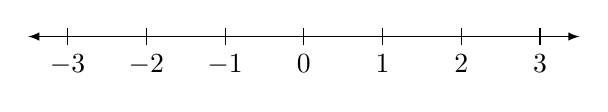
\begin{tikzpicture}
\draw[latex-latex] (-3.5,0) -- (3.5,0) ; %edit here for the axis
\foreach \x in  {-3,-2,-1,0,1,2,3} % edit here for the vertical lines
\draw[shift={(\x,0)},color=black] (0pt,3pt) -- (0pt,-3pt);
\foreach \x in {-3,-2,-1,0,1,2,3} % edit here for the numbers
\draw[shift={(\x,0)},color=black] (0pt,0pt) -- (0pt,-3pt) node[below]
{$\x$};
\end{tikzpicture}
\end{center}

\subsection{Irrational numbers}
\label{sec:org3b3a6ce}
There is no rational number x with the property that \(x^2 = 2\). \(x\) cannot be properly described by any rational number. However, the real number \(\sqrt{2}\) has this property. There are many real numbers that are not rational. Such numbers are called irrational numbers and some important examples are the constants \(\pi\) and \(e\).

\[x \text{ is irrational means that } x \in \mathbb{R} \setminus \mathbb{Q}\]

\newpage

\subsection{Intervals}
\label{sec:orgcad034f}
Intervals are special subsets of real number.
\\[0pt]

For \(a, b \in \mathbb{R}, a < b\), we use the notation:

\[\text{1. } (a, b] = \{x \in \mathbb{R}, a < x \le b\}\]

\begin{center}
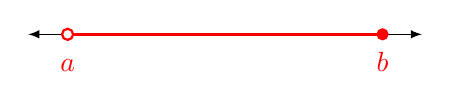
\begin{tikzpicture}

% The number line
\draw[latex-latex] (-2.5,0) -- (2.5,0);

% The thick line
\draw[very thick, color=red] (-2,0) -- (2,0);

% The circles
\path [draw=red, fill=white, thick] (-2,0) circle (2pt);
\path [draw=red, fill=red] (2,0.0) circle (2pt);

% The labels
\node[below, color=red] at (-2,-0.2) {$a$};
\node[below, color=red] at (2,-0.1){$b$};

\end{tikzpicture}
\end{center}




\[\text{2. } [a, b) = \{x \in \mathbb{R}, a \le x < b\}\]

\begin{center}
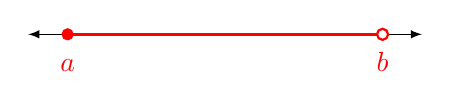
\begin{tikzpicture}

% The number line
\draw[latex-latex] (-2.5,0) -- (2.5,0);

% The thick line
\draw[very thick, color=red] (-2,0) -- (2,0);

% The circles
\path [draw=red, fill=red] (-2,0) circle (2pt);
\path [draw=red, fill=white, thick] (2,0.0) circle (2pt);

% The labels
\node[below, color=red] at (-2,-0.2) {$a$};
\node[below, color=red] at (2,-0.1){$b$};

\end{tikzpicture}
\end{center}




\[\text{3. } [a, b] = \{x \in \mathbb{R}, a \le x \le b\}\]

\begin{center}
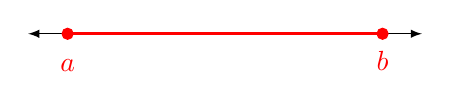
\begin{tikzpicture}

% The number line
\draw[latex-latex] (-2.5,0) -- (2.5,0);

% The thick line
\draw[very thick, color=red] (-2,0) -- (2,0);

% The circles
\path [draw=red, fill=red] (-2,0) circle (2pt);
\path [draw=red, fill=red] (2,0.0) circle (2pt);

% The labels
\node[below, color=red] at (-2,-0.2) {$a$};
\node[below, color=red] at (2,-0.1){$b$};

\end{tikzpicture}
\end{center}




\[\text{4. } (a, b) = \{x \in \mathbb{R}, a < x < b\}\]

\begin{center}
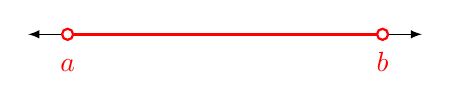
\begin{tikzpicture}

% The number line
\draw[latex-latex] (-2.5,0) -- (2.5,0);

% The thick line
\draw[very thick, color=red] (-2,0) -- (2,0);

% The circles
\path [draw=red, fill=white, thick] (-2,0) circle (2pt);
\path [draw=red, fill=white, thick] (2,0.0) circle (2pt);

% The labels
\node[below, color=red] at (-2,-0.2) {$a$};
\node[below, color=red] at (2,-0.1){$b$};

\end{tikzpicture}
\end{center}




\begin{center}
\begin{align*}
\text{5. } &[a, \infty) = \{x \in \mathbb{R}, a \le x\} \\
&(a, \infty) = \{x \in \mathbb{R}, a < x\} \\
&(-\infty, b] = \{x \in \mathbb{R}, x \le b\} \\
&(-\infty, b) = \{x \in \mathbb{R}, x < b\} \\
&(-\infty, \infty) = \mathbb{R}
\end{align*}
\end{center}

\newpage


\section{Logic}
\label{sec:orgeada2ea}


\subsection{Statements}
\label{sec:orgcb916c3}
In Maths, a statement is either true or false. A statement in maths cannot be both true and false, or be neither true nor false.
\\[0pt]

Examples:

\[4 < 7 \rightarrow \text{True}\]
\[4 = 7 \rightarrow \text{False}\]
\[\text{There are infinitely many prime numbers.} \rightarrow \text{True}\]
\[\text{All prime numbers are odd.} \rightarrow \text{False}\]
\[\text{The real part of every non-trivial zero of the Riemann zeta function is 1/2.} \rightarrow \text{?}\]

\subsection{Examples of non-statements}
\label{sec:orgf608324}

\[4.\]
\[\text{Hello!}\]
\[\text{This sentence is false.}\]

\subsection{Negating a statement}
\label{sec:org247ac1b}
The negation \(not\) \(P\) of a statement \(P\), is a statement that is false when \(P\) is true and is true when \(P\) is false.
\\[0pt]

Truth table:

\begin{center}
\begin{tabular}{ |c|c| }
\hline
P & not P \\
\hline
T & F \\
\hline
\end{tabular}
\end{center}




More examples:

\begin{flushleft}
\begin{tabular}{ | m{15em} | m{15em} | }
\hline
P & not P \\
\hline
x = 7 & x $\neq$ 7 \\
\hline
x < 7 & x $\ge$ 7 \\
\hline
All NTU students are younger than 30. & There exists an NTU student that is at least 30. \\
\hline
There exists a professor in NTU that is sane. & All professors in NTU are insane. \\
\hline
\end{tabular}
\end{flushleft}

\subsection{"For all" statements}
\label{sec:orgfbca6e2}
"For all" is represented by "\(\forall\)".

\subsection{"There exists" statements}
\label{sec:org431e11d}
"There exists" is represented by "\(\exists\)".

\subsection{Interactions between "for all" and "there exists" statements}
\label{sec:org640407b}
In general, the negation of "\(\forall x \in A, P(x) \text{ is true}\)", is "\(\exists x \in A, P(x) \text{ is false}\)". Similarly, the negation of "\(\exists x \in A, P(x) \text{ is true}\)", is "\(\forall x \in A, P(x) \text{ is false}\)".


\section{Open sets}
\label{sec:orga7c46eb}
A set \(A \subset \mathbb{R}\) is open if for every \(x \in A\), there exists a \(\delta > 0\) such that \((x - \delta, x + \delta) \subset A\). The set \(A\) is not open when there exists \(x \in A\) such that for every \(\delta > 0\), \((x - \delta, x + \delta) \notin A\).
\\[0pt]

To make this definition easier to understand, let's assume \(\delta\) to be a very small number. Let's look at the set of \((3,5)\). If we pick a \(x\) value that is very close to the boundary, like 4.9999 (\(x \neq 5\) as the set doesn't include 5), there's still a value of \(\delta\) that is greater than 0 (\(\delta > 0\)) that can be added to 4.9999 that will not cause \((x + \delta)\) to exceed the bounding value. In this case, \(\delta\) would be 0.000001. Similarly, for the lower bound, we can pick a \(x\) value that is very close to the boundary, such as 3.0001 (\(x \neq 3\) as the set doesn't include 3), and there will still be a non-zero \(\delta\) that is greater than 0 (\(\delta > 0\)) that can be subtracted from \(x\) that will not cause \((x - \delta)\) to be lower than the lower bound. In this case, \(\delta\) would be 0.00001. Hence, \((3,5)\) would be an open set.
\\[0pt]

Now, let's look at the set of \([3,5]\). If we pick a \(x\) value that is at the boundary (remember that the set includes the boundaries), like 5, there's no value of \(\delta\) that is greater than 0 (\(\delta > 0\)) that can be added to 5 that will not cause \((x + \delta)\) to exceed the bounding value. Similarly, for the lower bound, if we pick a \(x\) value that is at the boundary (the set includes the boundaries), such as 3, and there's no value of \(\delta\) that is greater than 0 (\(\delta > 0\)) that can be subtracted from \(x\) that will not cause \((x - \delta)\) to be lower than the lower bound. Hence, \((3,5)\) would not be an open set.
\\[0pt]

Examples (suppose \(a < b\)):

\[\text{1. } (a, b) \rightarrow \text{ Open}\]

\begin{center}
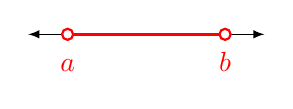
\begin{tikzpicture}

% The number line
\draw[latex-latex] (-1.5,0) -- (1.5,0);

% The thick line
\draw[very thick, color=red] (-1,0) -- (1,0);

% The circles
\path [draw=red, fill=white, thick] (-1,0) circle (2pt);
\path [draw=red, fill=white, thick] (1,0.0) circle (2pt);

% The labels
\node[below, color=red] at (-1,-0.2) {$a$};
\node[below, color=red] at (1,-0.1){$b$};

\end{tikzpicture}
\end{center}




\[\text{2. } (a, b] \rightarrow \text{ Not open}\]

\begin{center}
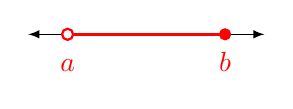
\begin{tikzpicture}

% The number line
\draw[latex-latex] (-1.5,0) -- (1.5,0);

% The thick line
\draw[very thick, color=red] (-1,0) -- (1,0);

% The circles
\path [draw=red, fill=white, thick] (-1,0) circle (2pt);
\path [draw=red, fill=red] (1,0.0) circle (2pt);

% The labels
\node[below, color=red] at (-1,-0.2) {$a$};
\node[below, color=red] at (1,-0.1){$b$};

\end{tikzpicture}
\end{center}




\[\text{3. } [a, b] \rightarrow \text{ Not open}\]

\begin{center}
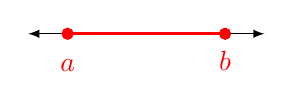
\begin{tikzpicture}

% The number line
\draw[latex-latex] (-1.5,0) -- (1.5,0);

% The thick line
\draw[very thick, color=red] (-1,0) -- (1,0);

% The circles
\path [draw=red, fill=red] (-1,0) circle (2pt);
\path [draw=red, fill=red] (1,0.0) circle (2pt);

% The labels
\node[below, color=red] at (-1,-0.2) {$a$};
\node[below, color=red] at (1,-0.1){$b$};

\end{tikzpicture}
\end{center}




\[\text{4. } (a, \infty) \rightarrow \text{ Open}\]

\begin{center}
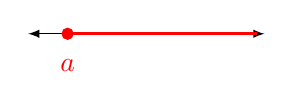
\begin{tikzpicture}

% The number line
\draw[latex-latex] (-1.5,0) -- (1.5,0);

% The thick line
\draw[very thick, color=red] (-1,0) -- (1.4,0);

% The circles
\path [draw=red, fill=red] (-1,0) circle (2pt);

% The labels
\node[below, color=red] at (-1,-0.2) {$a$};

\end{tikzpicture}
\end{center}




\[\text{5. } [a, \infty) \rightarrow \text{ Not open}\]

\begin{center}
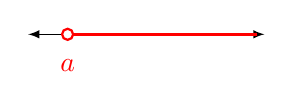
\begin{tikzpicture}

% The number line
\draw[latex-latex] (-1.5,0) -- (1.5,0);

% The thick line
\draw[very thick, color=red] (-1,0) -- (1.4,0);

% The circles
\path [draw=red, fill=white, thick] (-1,0) circle (2pt);

% The labels
\node[below, color=red] at (-1,-0.2) {$a$};

\end{tikzpicture}
\end{center}


\subsection{Not open sets}
\label{sec:orga4c66bc}
A set is \textbf{not open} means that \textbf{there exists \(x \in A\) such that for every \(\delta > 0\), \((x - \delta, x + \delta) \not\subset A\)}.




\section{Closed sets}
\label{sec:org940d7e0}
A set \(A \subset \mathbb{R}\) is closed if its "complement" \(\mathbb{R} \setminus A\) is open.

\newpage

Examples (suppose \(a < b\)):

\[\text{1. } (a, b) \rightarrow \text{ Not closed}\]
\[\mathbb{R} \setminus (a, b) = (-\infty, a] \cup [b, \infty) \text{ is not open. Hence } (a, b) \text{ is not closed.}\]

\[\text{2. } (a, b] \rightarrow \text{ Not closed}\]
\[\mathbb{R} \setminus (a, b] = (-\infty, a] \cup [b, \infty) \text{ is not open. Hence } (a, b] \text{ is not closed.}\]

\[\text{3. } [a, b] \rightarrow \text{Closed}\]
\[\mathbb{R} \setminus [a, b] = (-\infty, a) \cup (b, \infty) \text{ is open. Hence } [a, b] \text{ is closed.}\]

\[\text{4. } (a, \infty) \rightarrow \text{ Not closed}\]
\[\mathbb{R} \setminus (a, \infty) = (-\infty, a] \text{ is not open. Hence } (a, \infty) \text{ is not closed.}\]

\[\text{5. } [a, \infty) \rightarrow \text{ Closed}\]
\[\mathbb{R} \setminus [a, \infty) = (-\infty, a) \text{ is open. Hence } (a, \infty) \text{ is closed.}\]

\[\text{6. } \mathbb{R} \rightarrow \text{ Closed}\]
\[\mathbb{R} \setminus \mathbb{R} = \emptyset \text{ is open. Hence } \mathbb{R} \text{ is closed.}\]

\[\text{7. } \emptyset \rightarrow \text{ Closed}\]
\[\mathbb{R} \setminus \emptyset = \mathbb{R} \text{ is open. Hence } \emptyset \text{ is closed.}\]
\\[0pt]

From the examples, we can see that the set \((a, b]\) is neither open nor closed and the sets \(\mathbb{R}\) and \(\emptyset\) are both closed and open at the same time. \(\mathbb{R}\) and \(\emptyset\) are known as clopen sets, which are sets that are both closed and open. This means that open and closed sets are \textbf{not mutually exclusive} and both can happen at the same time.
\\[0pt]

In general, an open set is usually a set that does not include its bounding values while a closed set is a set that includes its bounding values, but this is not always the case, as seen from the sets \((a, b]\), \(\mathbb{R}\) and \(\emptyset\).


\section{Logical AND}
\label{sec:orgb84b2ac}
Given two statements \(P\) and \(Q\), the statement \(P\) \textbf{AND} \(Q\) is true when both \(P\) and \(Q\) are true, and false otherwise.
\\[0pt]

Truth table:

\begin{center}
\begin{tabular}{ |c|c|c| }
\hline
P & Q & P AND Q \\
\hline
T & T & T \\
\hline
T & F & F \\
\hline
F & T & F \\
\hline
F & F & F \\
\hline
\end{tabular}
\end{center}


\section{Logical OR}
\label{sec:orgd39ea75}
The statement \(P\) \textbf{OR} \(Q\) is false when \textbf{both} \(P\) and \(Q\) are false, and true otherwise.
\\[0pt]

Truth table:

\begin{center}
\begin{tabular}{ |c|c|c| }
\hline
P & Q & P OR Q \\
\hline
T & T & T \\
\hline
T & F & T \\
\hline
F & T & T \\
\hline
F & F & F \\
\hline
\end{tabular}
\end{center}

Examples:

\begin{center}
\begin{tabular}{ |c|c|c|c|c| }
\hline
P & Q & $not$ Q & (P AND $not$ Q) & $not$ (P AND $not$ Q) \\
\hline
T & T & F & F & T \\
\hline
T & F & T & T & F \\
\hline
F & T & F & F & T \\
\hline
F & F & T & F & T \\
\hline
\end{tabular}
\end{center}

\newpage


\section{Implications}
\label{sec:orga7b959d}
Many statements in maths have the form "if something, then something". For example:
\begin{itemize}
\item If \(x\) is an even integer, then \(x^2\) is an even integer.
\item If \(f(x)\) is differentiable at \(x = a\), then \(f(x)\) is continuous at \(x = a\).
\end{itemize}

We often use implications in our day-to-day life.
\begin{itemize}
\item If it rains, then I'll bring an umbrella.
\end{itemize}

\subsection{Notation}
\label{sec:orgc3db0a0}
The statement "if \(A\), then \(B\)" can also be expressed as \(A \Rightarrow B\), which means \(A\) implies \(B\).

\subsubsection{Example 1}
\label{sec:org621f90e}

\[x \text{ is an even integer. } \Rightarrow x^2 \text{ is an even integer.}\]

\subsubsection{Example 2}
\label{sec:orgeac8822}

If \(x > 0\) then \(x^2 > x^\frac{1}{2}\). The statement is false, as when \(x = 1\), \(x > 0\) but \(x^2 = x^\frac{1}{2}\). The implication mentioned above is false because it is possible for "\(x > 0\)" to be true without "\(x^2 > x^\frac{1}{2}\)" to be true. The first statement does not guarantee the second and hence the implication is false. This is usually demonstrated using a counterexample.

The truth value of the above implication does not "depend on \(x\)". It is irrelevant that \(x^2 > x^\frac{1}{2}\) for some \(x > 0\). The above implication is simply \textbf{false}.

\newpage

\subsubsection{Example 3}
\label{sec:org06126c3}

If \(p_k\) is the \(k \text{th}\) prime number, i.e.

\[p_1 = 2, p_2 = 3, p_3 = 5, p_4 = 7, p_5 = 11\]

And if \(n\) is a positive integer, then

\[1 + \prod_{k=1}^{n} p_k = 1 + p_1 \cdot ... \cdot p_n\]

Is also a prime number.


\begin{center}
\begin{tabular}{ c|c }
n & \(1 + \prod_{k=1}^{n} p_k\) \\
\hline
1 & \(1 + 2 = 3 \rightarrow \text{ prime}\) \\
2 & \(1 + 2 \cdot 3 = 7 \rightarrow \text{ prime}\) \\
3 & \(1 + 2 \cdot 3 \cdot 5 = 31 \rightarrow \text{ prime}\) \\
4 & \(1 + 2 \cdot 3 \cdot 5 \cdot 7 = 211 \rightarrow \text{ prime}\) \\
5 & \(1 + 2 \cdot 3 \cdot 5 \cdot 7 \cdot 11 = 2311 \rightarrow \text{ prime}\) \\
6 & \(1 + 2 \cdot 3 \cdot 5 \cdot 7 \cdot 11 \cdot 13 = 59,509 \rightarrow \textbf{ not prime}\)\\
\end{tabular}
\end{center}

Hence, the implication is \textbf{false}.

\newpage

\subsubsection{Example 4}
\label{sec:orgd8c4e73}

If \(a\) and \(b\) are positive real numbers, then:
\[\frac{a + b}{2} \ge \sqrt{ab}\]

\[\frac{a + b}{2} \text{ is the arithmetic mean of a and b.}\]
\[\sqrt{ab} \text{ is the geometric mean of a and b.}\]
\\[0pt]

The implication is \textbf{true}, as for \(a, b > 0\), we have
\begin{align*}
\frac{a + b}{2} - \sqrt{ab} &= \frac{a}{2} - \sqrt{ab} + \frac{b}{2} \\
&= (\sqrt{\frac{a}{2}} - \sqrt{\frac{b}{2}})^2 \\
&\ge 0
\end{align*}

\subsubsection{Example 5}
\label{sec:orgf93c842}

If \(x\) is a real number and \(x^2 < 0\), then \(x\) is a pink elephant. This statement is \textbf{true}.
\\[0pt]

If we let:

\[A = \{x \in \mathbb{R} : x^2 < 0\} = \emptyset\]

The last statement can be phrased as "for all \(x \in A, x\) is a pink elephant". The negation of this statement would be "there exists \(x \in A\), such that \(x\) is not a pink elephant". Since the negation of the original statement is \textbf{false}, the original statement must be \textbf{true}.

\newpage

\subsection{Another way to think about implications}
\label{sec:orgb28d8a8}
The implication \(P \Rightarrow Q\) is another way of saying \(not (\text{P AND } not \text{ Q})\).

\begin{center}
\begin{tabular}{ |c|c|c| }
\hline
P & Q & $not$ (P AND $not$ Q) \\
\hline
T & T & T \\
\hline
T & F & F \\
\hline
F & T & T \\
\hline
F & F & T \\
\hline
\end{tabular}
\end{center}

\[\downarrow\]

\begin{center}
\begin{tabular}{ |c|c|c| }
\hline
P & Q & $P \Rightarrow Q$ \\
\hline
T & T & T \\
\hline
T & F & F \\
\hline
F & T & T \\
\hline
F & F & T \\
\hline
\end{tabular}
\end{center}


\section{Equivalences}
\label{sec:orgf0186f1}
An implication has a "direction". For example, the implication \(x = 2 \Rightarrow x^2 = 4\) is \textbf{true} but if we turn it around, \(x^2 = 4 \Rightarrow x = 2\), we get something \textbf{false}.
\\[0pt]

If we instead consider the implication \(x = 2 \text{ or } x = -2 \Rightarrow x^2 = 4\), which is still true, we see that the "reverse" implication \(x^2 = 4 \Rightarrow x = 2 \text{ or } x = -2\) also holds. Hence, the two statements "\(x = 2 \text{ or } x = -2\)" and "\(x^2 = 4\)" are \textbf{equivalent}.
\\[0pt]

The statement \((P \Rightarrow Q)\) and \((Q \Rightarrow P)\) can be written as \(P \Leftrightarrow Q\). In this case, we say that \(P\) and \(Q\) are equivalent, or \(P\) if and only if \(Q\).

\newpage


\section{Contrapositive statement}
\label{sec:org62222e0}
Suppose that you \textbf{know} that the implication "if it rains, then your lecturer carries an umbrella" is a \textbf{true} statement. One day, you see your lecturer not carrying an umbrella, so you conclude that "if your lecturer does not carry an umbrella, then it does not rain".

The statements \(P \Rightarrow Q\) and \(not \text{ } Q \Rightarrow not \text{ } P\) are equivalent.

\begin{center}
\begin{tabular}{ |c|c|c|c|c|c| }
\hline
P & Q & $P \Rightarrow Q$ & $not$ Q & $not$ P & $not$ Q $\Rightarrow not$ P \\
\hline
T & T & T & F & F & T\\
\hline
T & F & F & T & F & F \\
\hline
F & T & T & F & T & T \\
\hline
F & F & T & T & T & T \\
\hline
\end{tabular}
\end{center}


\section{Functions}
\label{sec:orgb6f0c41}

\subsection{Definition}
\label{sec:orgbe4c6c3}
Consider two sets \(A\) and \(B\). A \textbf{function} \(f : A \rightarrow B\) is a rule that assigns to each element \(x \in A\) exactly one element \(f(x) \in B\) called the value of the function \(f\) at the point \(x\).
\\[0pt]

Put simply, a function takes a set of inputs, \(A\) and returns a set of outputs \(B\). One input can only have one output.
\\[0pt]

The set \(A\) is called the \textbf{domain} of \(f\), and \(B\) is called the \textbf{codomain} of \(f\). We also say that \(f : A \rightarrow B\) is a function \textbf{from} A \textbf{to} B.
\\[0pt]

\subsubsection{Example 1}
\label{sec:orgc6f100b}

\[f : \mathbb{R} \rightarrow \mathbb{R}, f(x) = x^2\]
\[f(1) = 1, f(-2) = 4\]

\newpage

\subsubsection{Example 2}
\label{sec:org74e253a}

Let \(A = \{\text{Homer}, \text{Marge}, \text{Bart}, \text{Lisa}, \text{Maggie}\}\) and define \(f : A \rightarrow \mathbb{N}\) by \(f(x) = \text{the age of } x \text{ in years.}\)

\[f(\text{Homer}) = 38\]
\[f(\text{Marge}) = 34\]
\[f(\text{Bart}) = 10\]
\[f(\text{Lisa}) = 8\]
\[f(\text{Maggie}) = 1\]

\[f(\text{Ned Flanders}) = \text{undefined}\]
\[\text{Ned Flanders} \notin A\]


\subsubsection{Important note}
\label{sec:org2961329}
For a function \(f\) with domain \(A, f(x)\) is only defined for \(x \in A\).
\\[0pt]

So for a function:
\[f : [0, \infty) \rightarrow \mathbb{R}\]
\[f(x) = x^2\]

\(f(-2) \neq 4\), instead \(f(-2) = \text{undefined}\) as \(f(x)\) is only defined for \(x \in A\).

\newpage

\subsection{Sequences}
\label{sec:org93762f2}

\subsubsection{Definition}
\label{sec:orgb0d10b6}
A function \(f : A \rightarrow \mathbb{R}\) where \(A\) is a subset of \(\mathbb{N}\) is called a \textbf{sequence}.

\begin{enumerate}
\item Example 1
\label{sec:org34e95a0}

The function \(f: \mathbb{N} \rightarrow \mathbb{R}\) defined by \(f(n) = 1 + \frac{(-1)^n}{n}\) is a sequence. We have:

\[f(1) = 1 + \frac{-1}{1} = 0, f(2) = 1 + \frac{1}{2} = \frac{3}{2}, f(3) = 1 + \frac{-1}{3} = \frac{2}{3}, \text{ etc.}\]

For sequences, we often use the notation \(a_n\) instead of \(f(n)\) and
\[(a_n), (a_n)_{n=1}^{\infty}, (a_1, a_2, a_3, ...), \text{ etc. instead of } f\]

\item Example 2
\label{sec:orgaf350ca}

The sequence in the example 1 would more commonly be described as
\[(a_n)_{n=1}^{\infty}, \text{ where } a_1 = 1 + \frac{-1}{1} = 0, a_2 = 1 + \frac{1}{2} = \frac{3}{2}, a_3 = 1 + \frac{-1}{3} = \frac{2}{3}, \text{ etc.}\]

\newpage
\end{enumerate}

\subsection{Different ways of describing functions}
\label{sec:org304379b}
A function can be described in any way. In fact, just using words is perfectly fine as long as the meaning is clear and unambiguous. Some particularly common ways are:
\\[0pt]

\textbf{Explicit formulae} like:

\begin{align*}
f(x) &= sin(1+x^3), \\
g(y) &= \frac{1+y}{1-y}, \\
a_n &= 2^n.
\end{align*}

\textbf{Implicit formulae} like:

\[\sin g(t) = t, \qquad -\pi \le g(t) \le \frac{\pi}{2},\]

\textbf{Recurrent formulae} for a sequence, like:

\[a_1 = 2, a_{n+1} = 2a_n,\]
\[\text{so } a_1 = 2, a_2 = 2a_1 = 4, a_3 = 2a_3 = 8, \text{ etc.}\]
\[a_1 = 1, a_2 = 2, a_{n+1} = a_n + a_{n-1}\]
\[\text{so } a_1 = 1, a_2 = 2, a_3 = a_2 + a_1 = 3, a_4 = a_3 + a_2 = 5, \text{ etc.}\]


\subsection{The graph of a function}
\label{sec:orgc4a412a}
A function \(f : A \rightarrow \mathbb{R}\) where \(A \subset \mathbb{R}\) can be represented by its \textbf{graph}.

The graph of \(f : A \rightarrow \mathbb{R}\) is formally defined as a set of pairs \((x, y)\).

\[G_f = \{(x, f(x)) : x \in A\}\]

\newpage

\subsection{The domain of a function}
\label{sec:org4764504}
For a function \(f : A \rightarrow B\), the set \(A\) is called the \textbf{domain} of \(f\). Note that the domain is part of the definition of a function, so:

\[f : \mathbb{R} \rightarrow \mathbb{R} \quad f(x) = x^2, \text{ and } g:[0, \infty] \rightarrow \mathbb{R} \quad g(x) = x^2\]

Are \textbf{different} functions.
\\[0pt]

Below is the graph of \(\color{blue} f(x)\) versus \(\color{red} g(x)\):
\\[0pt]

\begin{center}
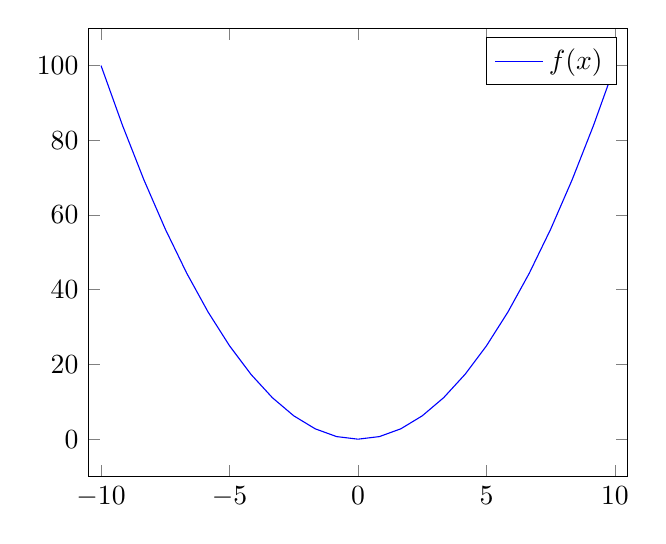
\begin{tikzpicture}
\begin{axis}[xmin = -10.5, xmax = 10.5]
\addplot[domain = -10:10, color = blue]{x^2};
\addlegendentry{\(f(x)\)}
\end{axis}
\end{tikzpicture}
\[\]

\begin{tikzpicture}
\begin{axis}[xmin = -10.5,xmax = 10.5]
\addplot[domain= 0:10, color = red]{x^2};
\addlegendentry{\(g(x)\)}
\end{axis}
\end{tikzpicture}
\end{center}

\subsubsection{The natural domain of a function}
\label{sec:org318bd19}
Usually, we will simply state an expression for \(f\) without saying what the domain is. For example \(f(x) = \sqrt{x-1}\), where the natural domain of \(f\) is \(\{x : x - 1 \ge 0\} = [1, \infty)\).

If we don't say anything about the domain, we will assume that it is the largest set \(A\), for which \(f(x)\) 'makes sense' when \(x \in A\). We also call this the \textbf{natural domain} of \(f\).

\subsection{Image and range of a function}
\label{sec:org0c7fc82}

\subsubsection{Definition}
\label{sec:org3bac71d}
Consider a function \(f : A \rightarrow B\).
\\[0pt]

For \(K \subset A\), the set \(f(K) = \{f(x) : x \in K\} \subset B\), is called the \textbf{image} of the set K. The image of \(f(A)\) of the whole domain \(A\) is called the range of the function \(f\).

\subsubsection{Example 1}
\label{sec:orgb3aff64}
\[\text{Let } A = \{\text{Homer}, \text{Marge}, \text{Bart}, \text{Lisa}, \text{Maggie}\}\]
\[\text{and define } f : A \rightarrow \mathbb{N} \text{ by } f(x) = \text{ the age of } x\]
\[\text{Also, let } K = \{\text{Bart}, \text{Lisa}, \text{Maggie}\}.\]
\\[0pt]

Remember that:

\[f(\text{Homer}) = 39\]
\[f(\text{Marge}) = 34\]
\[f(\text{Bart}) = 10\]
\[f(\text{Lisa}) = 8\]
\[f(\text{Maggie}) = 1\]
\\[0pt]

Then the "range of \(f\)" \(= f(A) = \{f(x) : x \in A\} = \{38, 34, 10, 8, 1\}\)
\[f(K) = \{f(x): x \in K\} = \{10, 8, 1\}\]

\subsubsection{Example 2}
\label{sec:orga3fa213}

\[f(x) = \sqrt{1-x^2}\]
\\[0pt]

Domain = \(\{x: 1 - x^2 \ge 0\} = \{ x : x^2 \le 1\} = [-1,1]\)
\\[0pt]

Range = \(\{\sqrt{1 - x^2} : x \in [-1, 1] = [0, 1]\}\)

\newpage

\section{Properties of functions}
\label{sec:org6f24de5}

\subsection{Increasing and decreasing functions}
\label{sec:org4f319d5}

\subsubsection{Definition}
\label{sec:org898c059}
A function \(f : A \rightarrow \mathbb{R}\) where \(A \subset \mathbb{R}\), is said to be:

\[\text{\textbf{Increasing} if } x_1, x_2 \in A, x_1 < x_2 \Rightarrow f(x_1) \le f(x_2)\]
\[\text{\textbf{Decreasing} if } x_1, x_2 \in A, x_1 < x_2 \Rightarrow f(x_1) \ge f(x_2)\]
\[\textbf{Monotonic } \text{if it is either increasing or decreasing.}\]

Furthermore, if \(B \subset A\), we say that \(f\) is increasing/decreasing/monotonic \textbf{on B} if either of the above conditions hold of \(x_1, x_2 \in B\).

\subsection{Strictly increasing and decreasing functions}
\label{sec:orgb67f729}

\subsubsection{Definition}
\label{sec:org0374fed}
A function \(f : A \rightarrow \mathbb{R} (A \subset \mathbb{R})\) is said to be:

\[\text{\textbf{Strictly increasing} if } x_1, x_2 \in A, x_1 < x_2 \Rightarrow f(x_1) < f(x_2)\]
\[\text{\textbf{Strictly decreasing} if } x_1, x_2 \in A, x_1 < x_2 \Rightarrow f(x_1) > f(x_2)\]
\[\textbf{Monotonic } \text{if it is either increasing or decreasing.}\]

Furthermore, if \(B \subset A\), we say that \(f\) is strictly increasing/decreasing/monotonic \textbf{on B} if either of the above conditions hold of \(x_1, x_2 \in B\).

\newpage

\subsubsection{Examples}
\label{sec:org2cb9171}

\[f : \mathbb{R} \rightarrow \mathbb{R}, f(x) = x^2 \text{ is not increasing as:}\]
\[-1 < 0 \text{ but } f(-1) > f(0)\]
\\[0pt]

\[f : [0, \infty] \rightarrow \mathbb{R}, f(x) = x^2 \text{ is strictly increasing as:}\]
\[x_1, x_2 \in (0, \infty) \text{ and } x_1 < x_2 \Rightarrow f(x_1) < f(x_2)\]
\\[0pt]

\[f : \mathbb{R} \rightarrow \mathbb{R}, f(x) = 1 \text{ is increasing}\]
\[x_1, x_2 \in \mathbb{R} \text{ and } x_1 < x_2 \Rightarrow f(x_1) \le f(x_2)\]
\[\text{But not strictly increasing as:}\]
\[0, 1 \in \mathbb{R} \text{ and } 0 < 1 \text{ but } f(0) = f(1)\]


\subsection{Bounded functions}
\label{sec:orgdb9501d}

\subsubsection{Definition}
\label{sec:org2702b36}
A function \(f : A \rightarrow \mathbb{R}\) is \textbf{bounded} if there exists a \(M > 0\) such that \(|f(x)| \le M, \text{ for all } x \in A\).
\\[0pt]

In simpler terms, a function that is bounded is a function that doesn't approach \(+\infty\) or \(-\infty\).
\\[0pt]

\textbf{Note that} \(|f(x)| \le M \Leftrightarrow - M \le f(x) \le M\).
\\[0pt]

A function that is not bounded is said to be \textbf{unbounded}. Furthermore, if \(B \subset A\), we say that \(f\) is bounded \textbf{on B} if the above inequality holds for all \(x \in B\).

\subsubsection{Example 1}
\label{sec:org1b096c5}
\[\sin x, \text{ } \cos x \text{ are bounded.}\]

The domain of \(\sin x\) is \(\mathbb{R}\). For all \(x \in \mathbb{R}\), we have \(|\sin x| \le 1\), so \(\sin x\) is bounded. The same is true for \(\cos x\).


\subsubsection{Example 2}
\label{sec:org9c51198}
\(x^2\) is bounded on the interval \([-2, 1]\), as for \(x \in [-2, 1]\) we have \(|x^2| \le 4\), so \(x^2\) is bounded on \([-2, 1]\).


\subsection{Locally bounded functions}
\label{sec:orgb62dd3b}

\subsubsection{Definition}
\label{sec:orgd0ec1f0}
A function \(f : A \rightarrow \mathbb{R}\) is \textbf{locally bounded at point} \(a \in A\) if there exists some \(\delta > 0\) such that \(f\) is bounded on \(A \cap (a - \delta, a + \delta)\).
\\[0pt]

A function that is \textbf{locally bounded} means that \(f\) is locally bounded at every \(a \in A\).

\subsubsection{Example 1}
\label{sec:org46a2465}

Given the definition of \(f\) below:

\[f : \mathbb{R} \setminus \{0\} \rightarrow \mathbb{R}, \text{ } f(x) = \frac{1}{x}\]

Show that \(f\) is locally bounded.
\\[0pt]

Let \(A\) be the domain of \(f\), i.e. \(A = \mathbb{R} \setminus \{0\}\), and suppose \(a \in A\).
\\[0pt]

Note that \(a \neq 0\), so \(a\) is within the domain of \(f\).
\\[0pt]

Let \(\delta = \frac{|a|}{2}, \text{ } M = \frac{2}{|a|}\), where \(M, \delta > 0\) and
\[|x| > \frac{|a|}{2}, \text{ for } x \in (a - \delta, a + \delta) \cap A.\]

Therefore,
\begin{align*}
|f(x)| = \frac{1}{|x|} &< \frac{1}{\frac{|a|}{2}} \\
&< \frac{2}{|a|} \\
&< M, \text{ for } x \in (a - \delta, a + \delta) \cap A
\end{align*}

Hence, \(f\) is bounded on \((a - \delta, a + \delta) \cap A\). Thus, \(f\) is locally bounded.


\subsubsection{Example 2}
\label{sec:orgabd4f88}

Given the definition of \(g\) below:

\begin{equation*}
g : \mathbb{R} \rightarrow \mathbb{R}, \text{ } g(x) = \begin{cases}
\frac{1}{x} & \text{ for } x \neq 0 \\
0 & \text{ for } x = 0
\end{cases}
\end{equation*}

Show that \(g\) is not locally bounded.
\\[0pt]

The definition of a locally bound function \(f\) is that for each \(a \in \mathbb{R}\), there exists \(\delta > 0\) such that \(f\) is bounded on \(a - \delta, a + \delta\).
\\[0pt]

So for a function \(f\) that is \textbf{not} locally bound, there exists some \(a \in \mathbb{R}\), such that \(f\) is not bounded on \(a - \delta, a + \delta\).
\\[0pt]

The domain \(A\) of \(g\) is \(\mathbb{R}\). Since \(0 \in A\), and for all \(\delta > 0, g\) is unbounded on \((0 - \delta, 0 + \delta) \cap A = (-\delta, \delta)\). That means \(g\) is not locally bounded at 0 and thus \(g\) is \textbf{not locally bounded}.


\subsection{Unbounded functions}
\label{sec:orgd7ba15a}

\subsubsection{Definition}
\label{sec:org43df6d4}
From the definition of a bounded function, which is "a function \(f : A \rightarrow \mathbb{R}\) is \textbf{bounded} if there exists a \(M > 0\) such that \(|f(x)| \le M, \text{ for all } x \in A\)".
\\[0pt]

A function that is not bounded is said to be \textbf{unbounded}, which is "\(f\) is bounded if for all \(M > 0\), there exists \(x \in A\) such that \(|f(x)| > M\)".

\newpage

\subsubsection{Example}
\label{sec:orga0db1a7}
Is the function \(f(x) = \frac{1}{x}\) bounded or unbounded?
\\[0pt]

For the graph below, \(\color{blue} y = f(x) = \frac{1}{x}\) is in blue, and \(\color{red} y = -M\) and \(\color{red} y = M\) are in red.
\\[0pt]

\begin{tikzpicture}
\begin{axis}[axis lines = middle, xmin = -10, xmax = 10, ymin = -10, ymax = 10]

% The graph of y = 1/x
\addplot[domain = -10:-0.1, color = blue]{1/x};
\addplot[domain = 0.1:10, color = blue]{1/x};

% The graph of y = M
\addplot[domain = -10:10, color = red]{3.5};

% The graph of y = -M
\addplot[domain = -10:10, color = red]{-3.5};

\end{axis}
\end{tikzpicture}
\\[0pt]

Domain of \(f = \mathbb{R} \setminus \{0\}\)
\\[0pt]

Let \(M > 0\), and take \(x = \frac{1}{2M}, x \in \mathbb{R} \setminus \{0\}\)

\[|f(x)| = \left|\frac{1}{\frac{1}{2M}} \right| = |2M| = 2M > 0\]

Hence, \(f\) is unbounded.

\newpage

\subsection{Odd and even functions}
\label{sec:org0d8db97}

\subsubsection{Definition}
\label{sec:org9e724d4}
A function \(f : A \rightarrow \mathbb{R}\) is said to be:

\[\text{\textbf{Odd} if } x \in A \Rightarrow -x \in A \text{ and } f(-x) = -f(x).\]

The graph of \(y = f(x)\) is symmetric about \$(0, 0).
\\[0pt]

\[\text{\textbf{Even} if } x \in A \Rightarrow -x \in A \text{ and } f(-x) = f(x).\]

The graph of \(y = f(x)\) is symmetric about the y-axis.


\subsection{Periodic functions}
\label{sec:org213b5f0}

\subsubsection{Definition}
\label{sec:org3dc0143}
A function \(f : \mathbb{R} \rightarrow \mathbb{R}\) is said to be \textbf{periodic} if there exists some \(T > 0\) such that \(f(x + T) = f(x), \text{ for all } x \in \mathbb{R}\).

The number \(T\) is called a \textbf{period} for \(f\).

\subsection{Examples}
\label{sec:orgb2d699c}
\(\sin x\) and \(\cos x\) are both periodic with period \(2\pi\).
\(\sin x\) is odd, \(\cos x\) is even.
\(x^2\) is even, \(x^3\) is odd.
\(e^x\) is neither odd nor even.
Given any function \(f(x)\), the function \(g(x) = f(|x|)\) is even.
\end{document}